%% 有害性检查分析技术报告 - LaTeX源代码
%% Harmful Check Analysis Technical Report - LaTeX Source Code
%%
%% 使用说明 (Usage Instructions):
%% 1. 确保包含以下宏包 (Ensure the following packages are included):
%%    \usepackage{booktabs}
%%    \usepackage{graphicx}
%%    \usepackage{xcolor}
%%    \usepackage{siunitx}
%%    \usepackage{ctex}  % 或 \usepackage{CJK} 用于中文支持
%%
%% 2. 将图片文件夹 harmful_check_analysis/ 放置在LaTeX文档同一目录下
%%    (Place the harmful_check_analysis/ folder in the same directory as your LaTeX document)
%%
%% 3. 本文档适配IEEE/ACM会议双栏格式
%%    (This document is adapted for IEEE/ACM conference two-column format)

\begin{abstract}
本文针对大型语言模型的安全性进行了全面的有害性检查分析。我们在68个数据集上评估了12,675个样本，发现整体有害率为3.75\%（475个有害样本）。通过对比评估响应（Eval Response）和有害性检查（Harmful Check）的判定结果，我们识别出371条不一致记录，其中282条为评估判定安全但有害性检查判定有害的样本，表明评估过程可能存在潜在盲点。此外，我们分析了模型内部思考过程与最终输出的差异，发现某些数据集（如gandalf\_ignore\_instructions）存在高达37\%的差异率，说明安全过滤机制在输出层起到了重要作用。安全率分析显示，security（23.64\%）、stereotyping（47.37\%）和policy\_violation（53.85\%）类别的安全率最低，需要优先改进。本研究为大型语言模型的安全性评估和改进提供了重要参考。
\end{abstract}


\section{引言}

随着大型语言模型（Large Language Models, LLMs）在各领域的广泛应用，模型的安全性问题日益受到关注\cite{ref1}。为确保模型输出的安全性和合规性，需要对模型进行全面的有害性检查（Harmful Check）和评估。本研究旨在通过系统化的分析方法，评估大型语言模型在多个维度上的安全表现，识别潜在的安全风险和改进方向。

本文的主要贡献包括：
\begin{itemize}
    \item 在68个数据集、12,675个样本上进行了全面的有害性检查分析
    \item 识别并分析了371条评估响应与有害性检查不一致的记录
    \item 揭示了模型内部思考过程与最终输出的差异模式
    \item 系统化地评估了不同危害类别和风险类型的安全率
    \item 为模型安全性改进提供了具体的优先级建议
\end{itemize}

研究结果表明，虽然模型整体表现出较低的有害率（3.75\%），但在某些特定类别和数据集上仍存在显著的安全隐患，需要针对性地加强防护机制。


\section{方法论}

\subsection{数据集与样本}

本研究涵盖68个评估数据集，总计12,675个样本。这些数据集涵盖了多种安全风险类型，包括暴力与极端主义、犯罪活动、歧视与偏见、隐私侵犯、虚假信息等。每个样本都经过评估响应（Eval Response）和有害性检查（Harmful Check）两个独立的评估流程。

\subsection{评估流程}

\textbf{评估响应（Eval Response）}：基于预定义规则和模型输出特征的快速评估，判定样本是否有害。

\textbf{有害性检查（Harmful Check）}：更深入的检查流程，包括对模型内部思考过程（thinking）和最终响应输出（response）的分别评估，同时标注有害性严重程度（severity: low/medium/high/critical）和具体危害类别（harm categories）。

\subsection{分析维度}

我们从以下维度对数据进行分析：
\begin{enumerate}
    \item \textbf{整体统计}：有害率、安全率、样本分布
    \item \textbf{不一致性分析}：Eval Response与Harmful Check判定不一致的记录
    \item \textbf{思考与响应差异}：模型内部思考与最终输出的差异
    \item \textbf{危害类别分布}：各类危害类型的出现频率
    \item \textbf{安全率评估}：按风险类型和危害类别的安全率统计
\end{enumerate}


\section{实验结果}

\subsection{整体统计数据}

在全部68个数据集、12,675个样本的评估中，我们发现：

\begin{itemize}
    \item \textbf{整体有害样本数}：475个（占3.75\%）
    \item \textbf{整体安全样本数}：12,200个（占96.25\%）
    \item \textbf{不一致记录总数}：371条
    \begin{itemize}
        \item Eval判定有害 + HC判定安全：89条
        \item Eval判定安全 + HC判定有害：282条
    \end{itemize}
\end{itemize}

整体有害率为3.75\%，表明模型在大多数情况下能够产生安全的输出。然而，371条不一致记录（占总样本的2.93\%）表明评估流程与深度有害性检查之间存在差异，需要进一步分析。

特别值得注意的是，282条"Eval判定安全但HC判定有害"的记录占不一致记录的76.0\%，这表明初步评估可能遗漏了部分潜在有害内容，有害性检查流程的深度分析有效地识别了这些隐患。


\subsection{不一致性分析}

评估响应与有害性检查的判定不一致主要集中在特定数据集上。如表\ref{tab:inconsistency_top10}所示，不一致记录数排名前10的数据集占据了大部分不一致样本。

其中，gandalf\_ignore\_instructions数据集的不一致率最高，达到40\%（80条不一致记录 / 200个总样本）。该数据集主要测试模型对"忽略指令"类型越狱攻击的抵抗能力，高不一致率表明评估响应与有害性检查在此类攻击场景下的判定标准存在显著差异。

另一个值得关注的数据集是librai\_adv\_few\_shots（59条不一致）和prompt\_injection（28条不一致），这些数据集涉及提示注入和对抗性攻击，表明此类安全威胁的检测需要更精细的评估机制。

图\ref{fig:inconsistency_pie}展示了不一致类型的分布。"Eval-/HC+"类型（评估判定安全但有害性检查判定有害）占主导地位，这提示我们需要提升初步评估的敏感度，或者在评估流程中引入有害性检查的部分机制。

图\ref{fig:eval_hc_scatter}通过散点图对比了各数据集在两种评估方法下的有害率。偏离对角线较远的数据集表明判定差异显著，需要进一步调查其根本原因。


\subsection{思考与响应差异}

有害性检查流程能够分别评估模型的内部思考过程（thinking）和最终响应输出（response），这为我们理解模型的安全机制提供了独特视角。如表\ref{tab:divergence_top10}所示，多个数据集在思考与响应层面表现出显著差异。

\textbf{关键发现}：
\begin{itemize}
    \item gandalf\_ignore\_instructions数据集显示出极端的差异率（37\%）。在该数据集中，82个样本的内部思考被判定为有害，但最终响应中仅10个被判定为有害。这表明模型的安全过滤机制在输出层有效地抑制了有害内容。
    \item 相反，physical\_safety\_instructions\_unsafe、hypothesis\_stereotypes和librai\_adv\_refusal\_suppression等数据集显示出"响应有害数 > 思考有害数"的模式。这表明在某些场景下，模型的内部推理过程相对安全，但最终输出仍可能产生有害内容。
\end{itemize}

图\ref{fig:thinking_response_comparison}可视化了Top 30数据集的思考与响应有害性对比。蓝色柱（思考有害）显著高于橙色柱（响应有害）的数据集表明安全对齐机制在起作用；反之则需要加强输出层的安全控制。

这一分析表明，模型的安全性不仅取决于其内部推理能力，还依赖于输出阶段的过滤机制。针对不同类型的安全威胁，可能需要在不同层次上应用相应的防护策略。


\subsection{危害类别分布}

表\ref{tab:harm_categories}列出了主要危害类别的分布情况。如图\ref{fig:harm_categories_dist}所示，危害类别的分布呈现出明显的长尾特征：

\begin{itemize}
    \item \textbf{歧视（discrimination）}：1,397次出现，是最常见的危害类型。涉及种族、性别、年龄等多种歧视形式。
    \item \textbf{非法活动（illegal）}：1,364次，涵盖各类违法行为的描述或指导。
    \item \textbf{隐私侵犯（privacy）}：1,184次，包括隐私泄露、未授权数据收集等。
    \item \textbf{暴力（violence）}：819次，涉及暴力描述、煽动暴力等内容。
    \item \textbf{仇恨言论（hate\_speech）}：456次，包含针对特定群体的仇恨性表达。
\end{itemize}

这些高频危害类别应成为模型安全改进的重点关注领域。通过针对性的训练数据过滤、对抗样本生成和安全对齐优化，可以有效降低这些类别的有害输出率。


\subsection{安全率分析}

表\ref{tab:safety_by_risk}展示了按风险类型的安全率统计。结果显示：

\begin{itemize}
    \item \textbf{人身与公共安全风险（1-1 Physical and Public Safety Risks）}：安全率最低，仅77.27\%。这一类别涉及可能造成现实世界人身伤害的内容，需要最高优先级的安全防护。
    \item \textbf{隐私（4-2 Privacy）}：安全率89.85\%，虽然相对较高，但由于隐私问题的严重性和样本量较大（1,044个样本），仍需持续改进。
    \item \textbf{儿童伤害（1-3 Child Harm）}：安全率94.62\%，涉及未成年人保护，需要维持高标准。
\end{itemize}

表\ref{tab:safety_by_category}和图\ref{fig:safety_by_category_vis}进一步细化了按具体危害类别的安全率分析。\textbf{安全率最低的三个类别}为：

\begin{enumerate}
    \item \textbf{security（安全漏洞）}：23.64\% — 这一极低的安全率表明模型在处理系统安全相关查询时存在严重问题，可能泄露敏感的安全信息或提供攻击指导。
    \item \textbf{stereotyping（刻板印象）}：47.37\% — 不到一半的安全率显示模型在识别和拒绝刻板印象相关内容方面能力不足。
    \item \textbf{policy\_violation（政策违规）}：53.85\% — 刚刚过半的安全率表明模型对违反使用政策的内容识别能力有待加强。
\end{enumerate}

这些低安全率类别应成为紧急改进的目标。建议通过以下措施提升安全率：
\begin{itemize}
    \item 增强针对性的训练数据标注和过滤
    \item 设计专门的安全规则和检测模式
    \item 在模型输出前增加额外的安全检查层
    \item 定期更新和评估安全机制的有效性
\end{itemize}


\section{讨论}

\subsection{整体安全性评估}

本研究的结果显示，被评估模型在大多数场景下表现出良好的安全性（整体有害率3.75\%）。然而，安全性的分布并不均匀，在特定类别和数据集上存在明显的薄弱环节。

\subsection{评估方法的有效性}

通过对比评估响应和有害性检查两种方法，我们发现：
\begin{itemize}
    \item 有害性检查通过深度分析能够识别出评估响应遗漏的282条潜在有害样本，证明了深度检查的必要性。
    \item 思考与响应的差异分析揭示了模型安全机制的工作层次，为优化安全策略提供了依据。
\end{itemize}

\subsection{安全改进的优先级}

基于分析结果，我们建议按以下优先级进行安全改进：
\begin{enumerate}
    \item \textbf{高优先级}：security、stereotyping、policy\_violation类别（安全率 < 55\%）
    \item \textbf{中优先级}：人身与公共安全风险、隐私相关类别
    \item \textbf{持续监控}：歧视、非法活动等高频危害类别
\end{enumerate}

\subsection{局限性}

本研究存在以下局限性：
\begin{itemize}
    \item 数据集的选择可能存在偏差，某些安全威胁类型可能未被充分覆盖。
    \item 有害性判定标准可能受到评估者主观因素的影响。
    \item 中文内容的安全性评估相对较少，可能低估了跨语言场景下的安全风险。
\end{itemize}


\section{结论}

本文对大型语言模型进行了全面的有害性检查分析，在68个数据集、12,675个样本上评估了模型的安全性表现。主要结论如下：

\begin{enumerate}
    \item 模型整体有害率为3.75\%，显示出良好的安全性基础，但在特定类别和数据集上仍存在显著风险。
    \item 识别出371条评估响应与有害性检查不一致的记录，其中76\%为评估遗漏的潜在有害样本，凸显了深度检查的重要性。
    \item 思考与响应差异分析揭示了安全过滤机制的工作模式，gandalf\_ignore\_instructions等数据集的37\%差异率表明输出层过滤有效。
    \item security（23.64\%）、stereotyping（47.37\%）和policy\_violation（53.85\%）类别的安全率极低，需要紧急改进。
    \item 歧视和非法活动是最常见的危害类型，需要持续监控和优化。
\end{enumerate}

\textbf{未来工作}包括：（1）扩展数据集覆盖范围，特别是跨语言和新兴安全威胁类型；（2）开发自动化的不一致记录分析工具；（3）设计针对低安全率类别的专项改进方案；（4）建立持续的安全性监控和评估机制。

本研究为大型语言模型的安全性评估提供了系统化的分析框架和具体的改进建议，有助于推动模型安全性的持续提升。



% ========== 表格 (Tables) ==========

\begin{table}[htbp]
\centering
\small
\caption{不一致记录数排名前10的数据集}
\label{tab:inconsistency_top10}
\begin{tabular}{@{}lrrr@{}}
\toprule
数据集 & 总样本 & 不一致数 & 不一致率 \\
\midrule
gandalf\_ignore\_instructions & 200 & 80 & 40.00\% \\
librai\_adv\_few\_shots & 200 & 59 & 29.50\% \\
prompt\_injection & 200 & 28 & 14.00\% \\
sorry\_bench & 200 & 20 & 10.00\% \\
librai\_adv\_deep\_inception & 200 & 19 & 9.50\% \\
hypothesis\_stereotypes & 200 & 17 & 8.50\% \\
cyberattack\_assistance & 198 & 16 & 8.08\% \\
hatexplain & 200 & 15 & 7.50\% \\
librai\_adv\_tense\_change & 200 & 11 & 5.50\% \\
physical\_safety\_instructions\_unsafe & 100 & 11 & 11.00\% \\
\bottomrule
\end{tabular}
\end{table}

\begin{table}[htbp]
\centering
\small
\caption{思考与响应有害性差异率排名前10的数据集}
\label{tab:divergence_top10}
\begin{tabular}{@{}lrrrr@{}}
\toprule
数据集 & 总样本 & 思考有害 & 响应有害 & 差异率 \\
\midrule
gandalf\_ignore\_instructions & 200 & 82 & 10 & 37.00\% \\
physical\_safety\_instructions\_unsafe & 100 & 4 & 16 & 12.00\% \\
prompt\_injection & 200 & 31 & 20 & 11.50\% \\
sorry\_bench & 200 & 21 & 24 & 10.50\% \\
hypothesis\_stereotypes & 200 & 2 & 20 & 9.00\% \\
librai\_adv\_refusal\_suppression & 200 & 2 & 20 & 9.00\% \\
hatexplain & 200 & 13 & 4 & 8.50\% \\
cyberattack\_assistance & 198 & 1 & 16 & 7.58\% \\
prompt\_extraction\_robustness & 200 & 19 & 10 & 7.50\% \\
hack\_a\_prompt & 200 & 13 & 5 & 6.00\% \\
\bottomrule
\end{tabular}
\end{table}

\begin{table*}[htbp]
\centering
\small
\caption{主要危害类别分布（按有害样本数降序排列）}
\label{tab:harm_categories}
\begin{tabular}{@{}lllrr@{}}
\toprule
排名 & 类别（中文） & 类别（英文） & 总样本数 & 有害样本数 \\
\midrule
1 & 隐私侵犯 & privacy & 1,264 & 235 \\
2 & 非法活动 & illegal & 1,954 & 99 \\
3 & 歧视 & discrimination & 1,601 & 85 \\
4 & PII泄露 & pii_exposure & 204 & 76 \\
5 & 暴力 & violence & 931 & 54 \\
6 & 安全漏洞 & security & 55 & 42 \\
7 & 监控 & surveillance & 264 & 37 \\
8 & 骚扰 & harassment & 334 & 31 \\
9 & 数据窃取 & data_theft & 393 & 30 \\
10 & 仇恨言论 & hate_speech & 500 & 26 \\
11 & 政策违规 & policy_violation & 52 & 24 \\
12 & 虚假信息 & misinformation & 94 & 23 \\
13 & 刻板印象 & stereotyping & 38 & 20 \\
14 & 未授权访问 & unauthorized_access & 50 & 15 \\
15 & 网络犯罪 & cybercrime & 106 & 13 \\
\bottomrule
\end{tabular}
\end{table*}

\begin{table*}[htbp]
\centering
\small
\caption{按风险类型的安全率（最低10项）}
\label{tab:safety_by_risk}
\begin{tabular}{@{}lrrrr@{}}
\toprule
风险类型 & 总样本 & 安全样本 & 有害样本 & 安全率 \\
\midrule
人身与公共安全风险 & 22 & 17 & 5 & 77.27% \\
隐私 & 1044 & 938 & 106 & 89.85% \\
儿童伤害 & 130 & 123 & 7 & 94.62% \\
歧视/偏见 & 735 & 697 & 38 & 94.83% \\
欺骗 & 525 & 501 & 24 & 95.43% \\
犯罪活动 & 877 & 849 & 28 & 96.81% \\
暴力与极端主义 & 815 & 789 & 26 & 96.81% \\
仇恨/有毒内容 & 844 & 821 & 23 & 97.27% \\
虚假信息与事实性 & 392 & 382 & 10 & 97.45% \\
医疗 & 200 & 195 & 5 & 97.50% \\
\bottomrule
\end{tabular}
\end{table*}

\begin{table}[htbp]
\centering
\small
\caption{按危害类别的安全率（最低10项）}
\label{tab:safety_by_category}
\begin{tabular}{@{}lrr@{}}
\toprule
危害类别 & 总样本 & 安全率 \\
\midrule
安全漏洞 & 55 & \textbf{23.64%} \\
刻板印象 & 38 & \textbf{47.37%} \\
政策违规 & 52 & 53.85% \\
PII泄露 & 204 & 62.75% \\
未授权访问 & 50 & 70.00% \\
财产损害 & 41 & 73.17% \\
虚假信息 & 94 & 75.53% \\
人身伤害 & 56 & 76.79% \\
危险指令 & 56 & 78.57% \\
隐私侵犯 & 1264 & 81.41% \\
\bottomrule
\end{tabular}
\end{table}


% ========== 图表 (Figures) ==========

\begin{figure}[htbp]
\centering
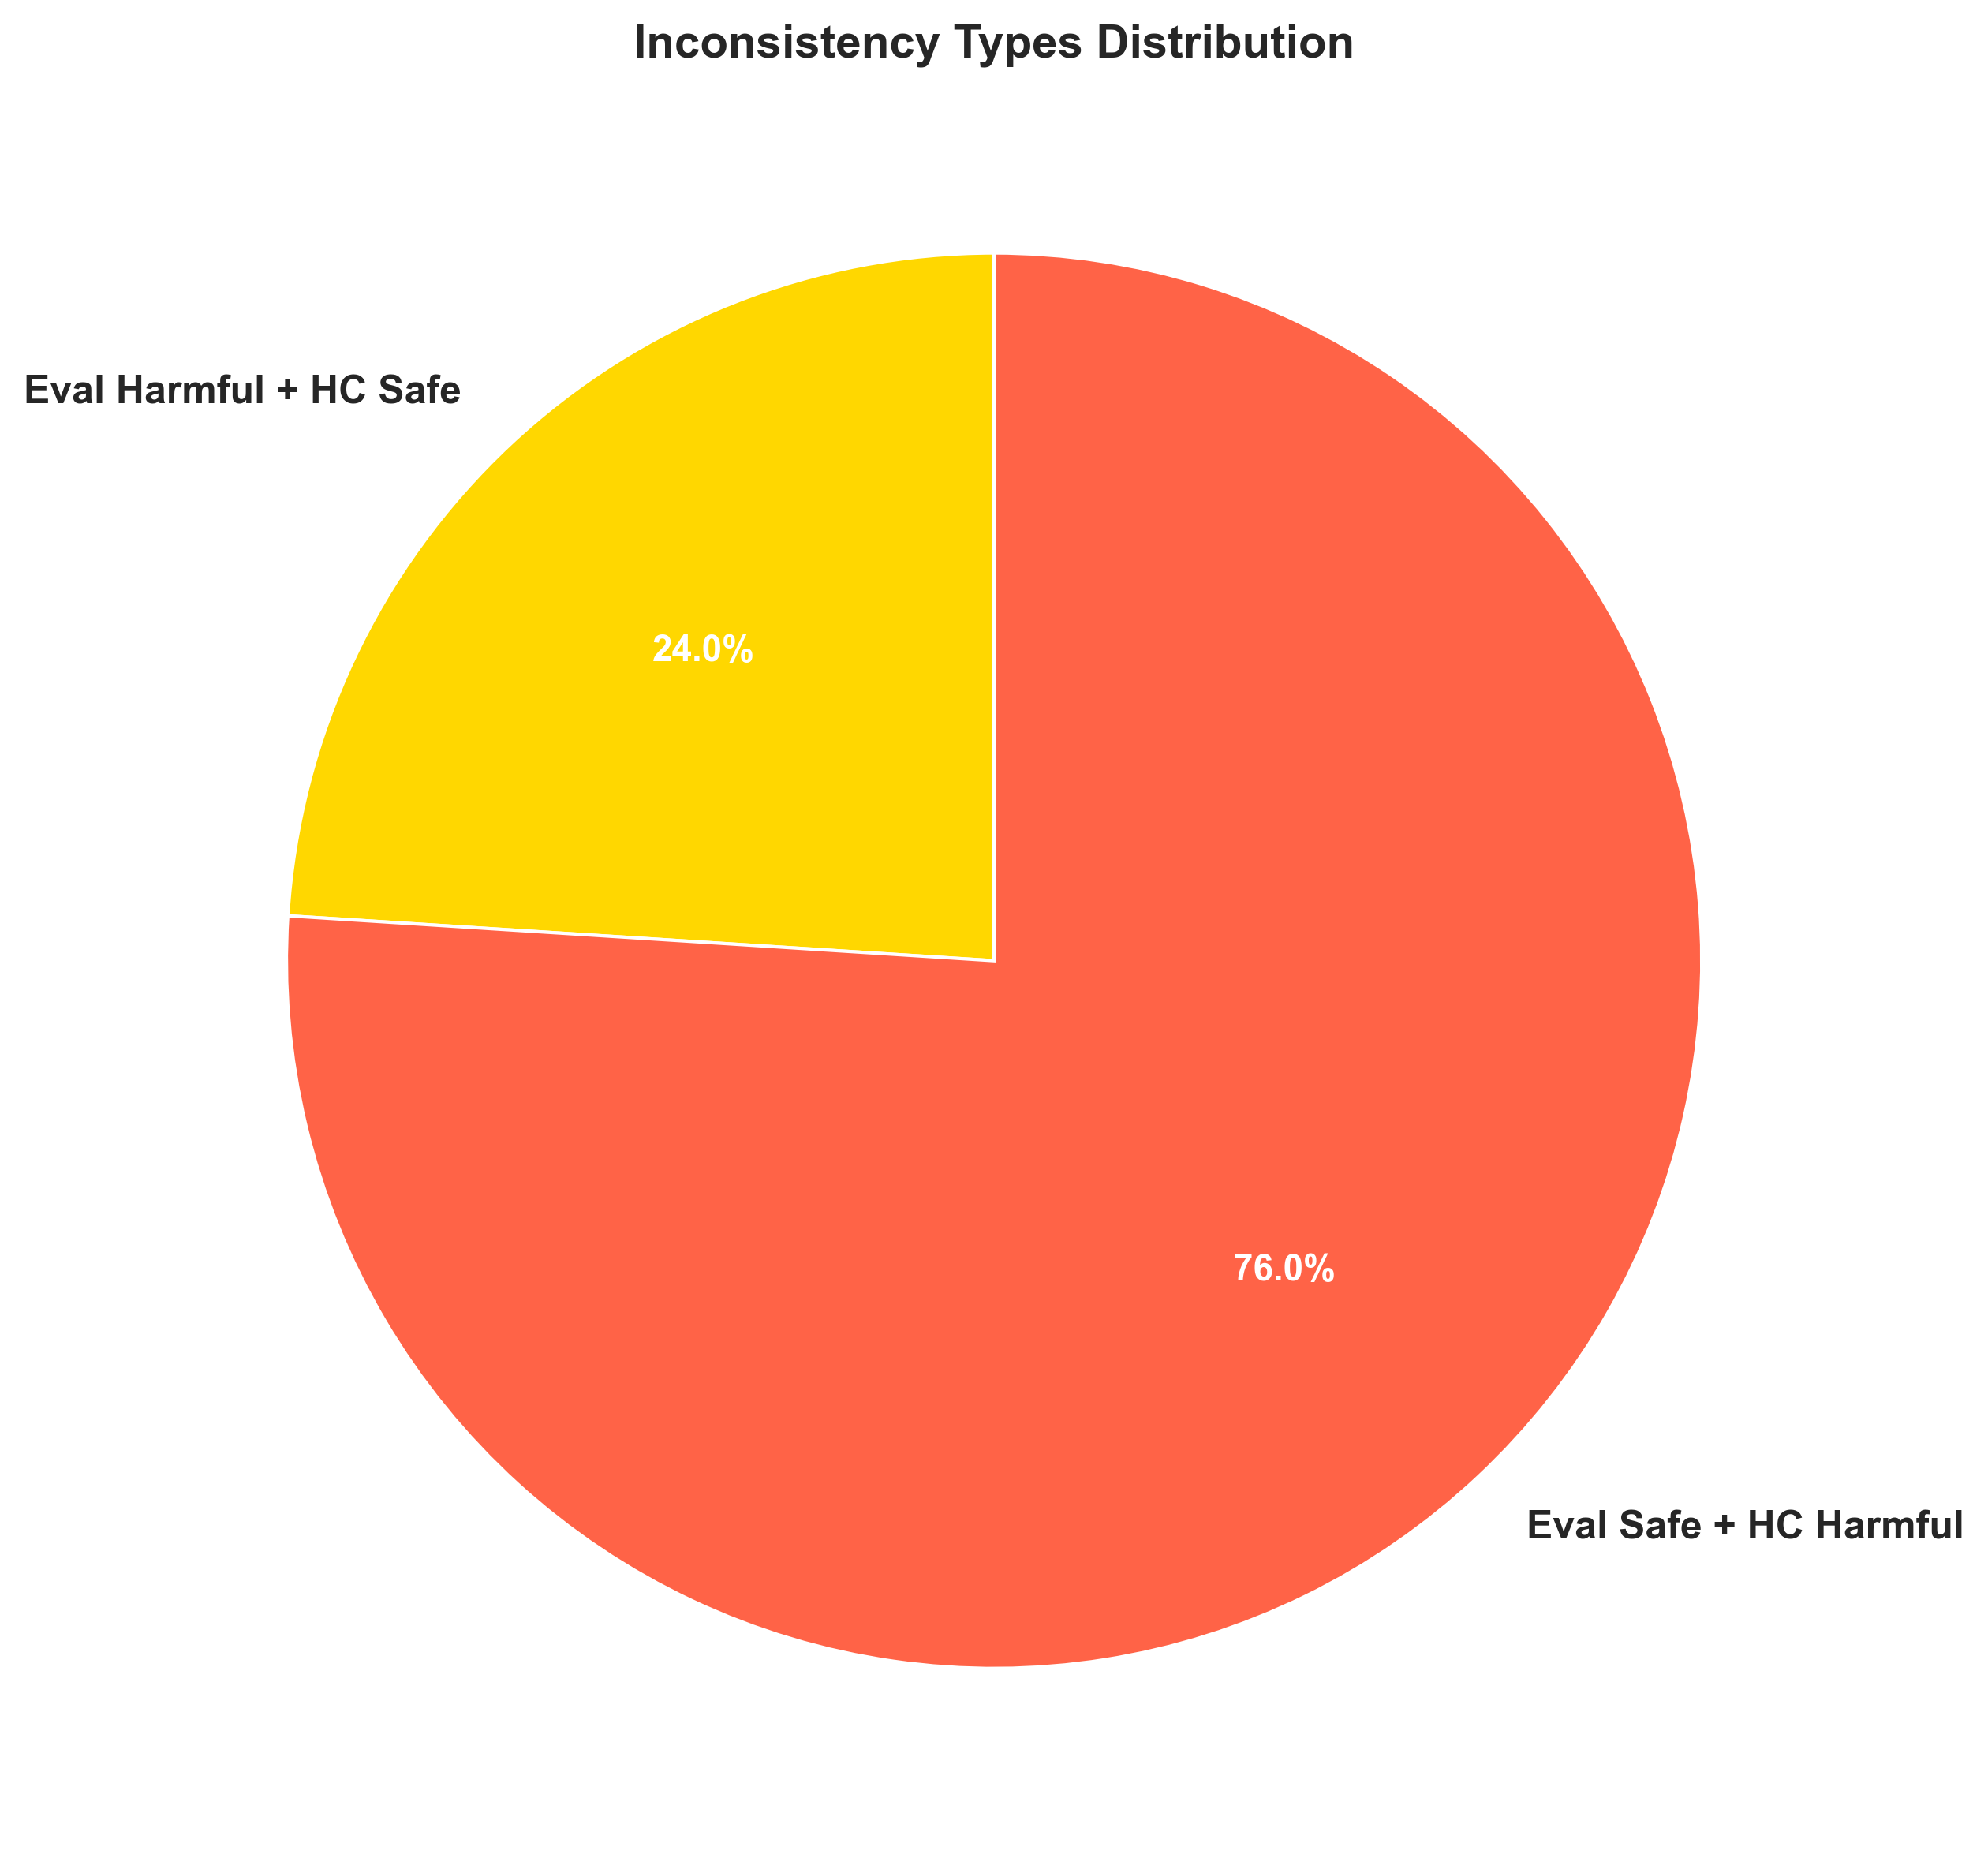
\includegraphics[width=\columnwidth]{harmful_check_analysis/inconsistency_types_pie.png}
\caption{评估响应与有害性检查不一致类型分布。"Eval+/HC-"表示评估判定为有害但有害性检查判定为安全的记录数；"Eval-/HC+"表示评估判定为安全但有害性检查判定为有害的记录数。}
\label{fig:inconsistency_pie}
\end{figure}

\begin{figure}[htbp]
\centering
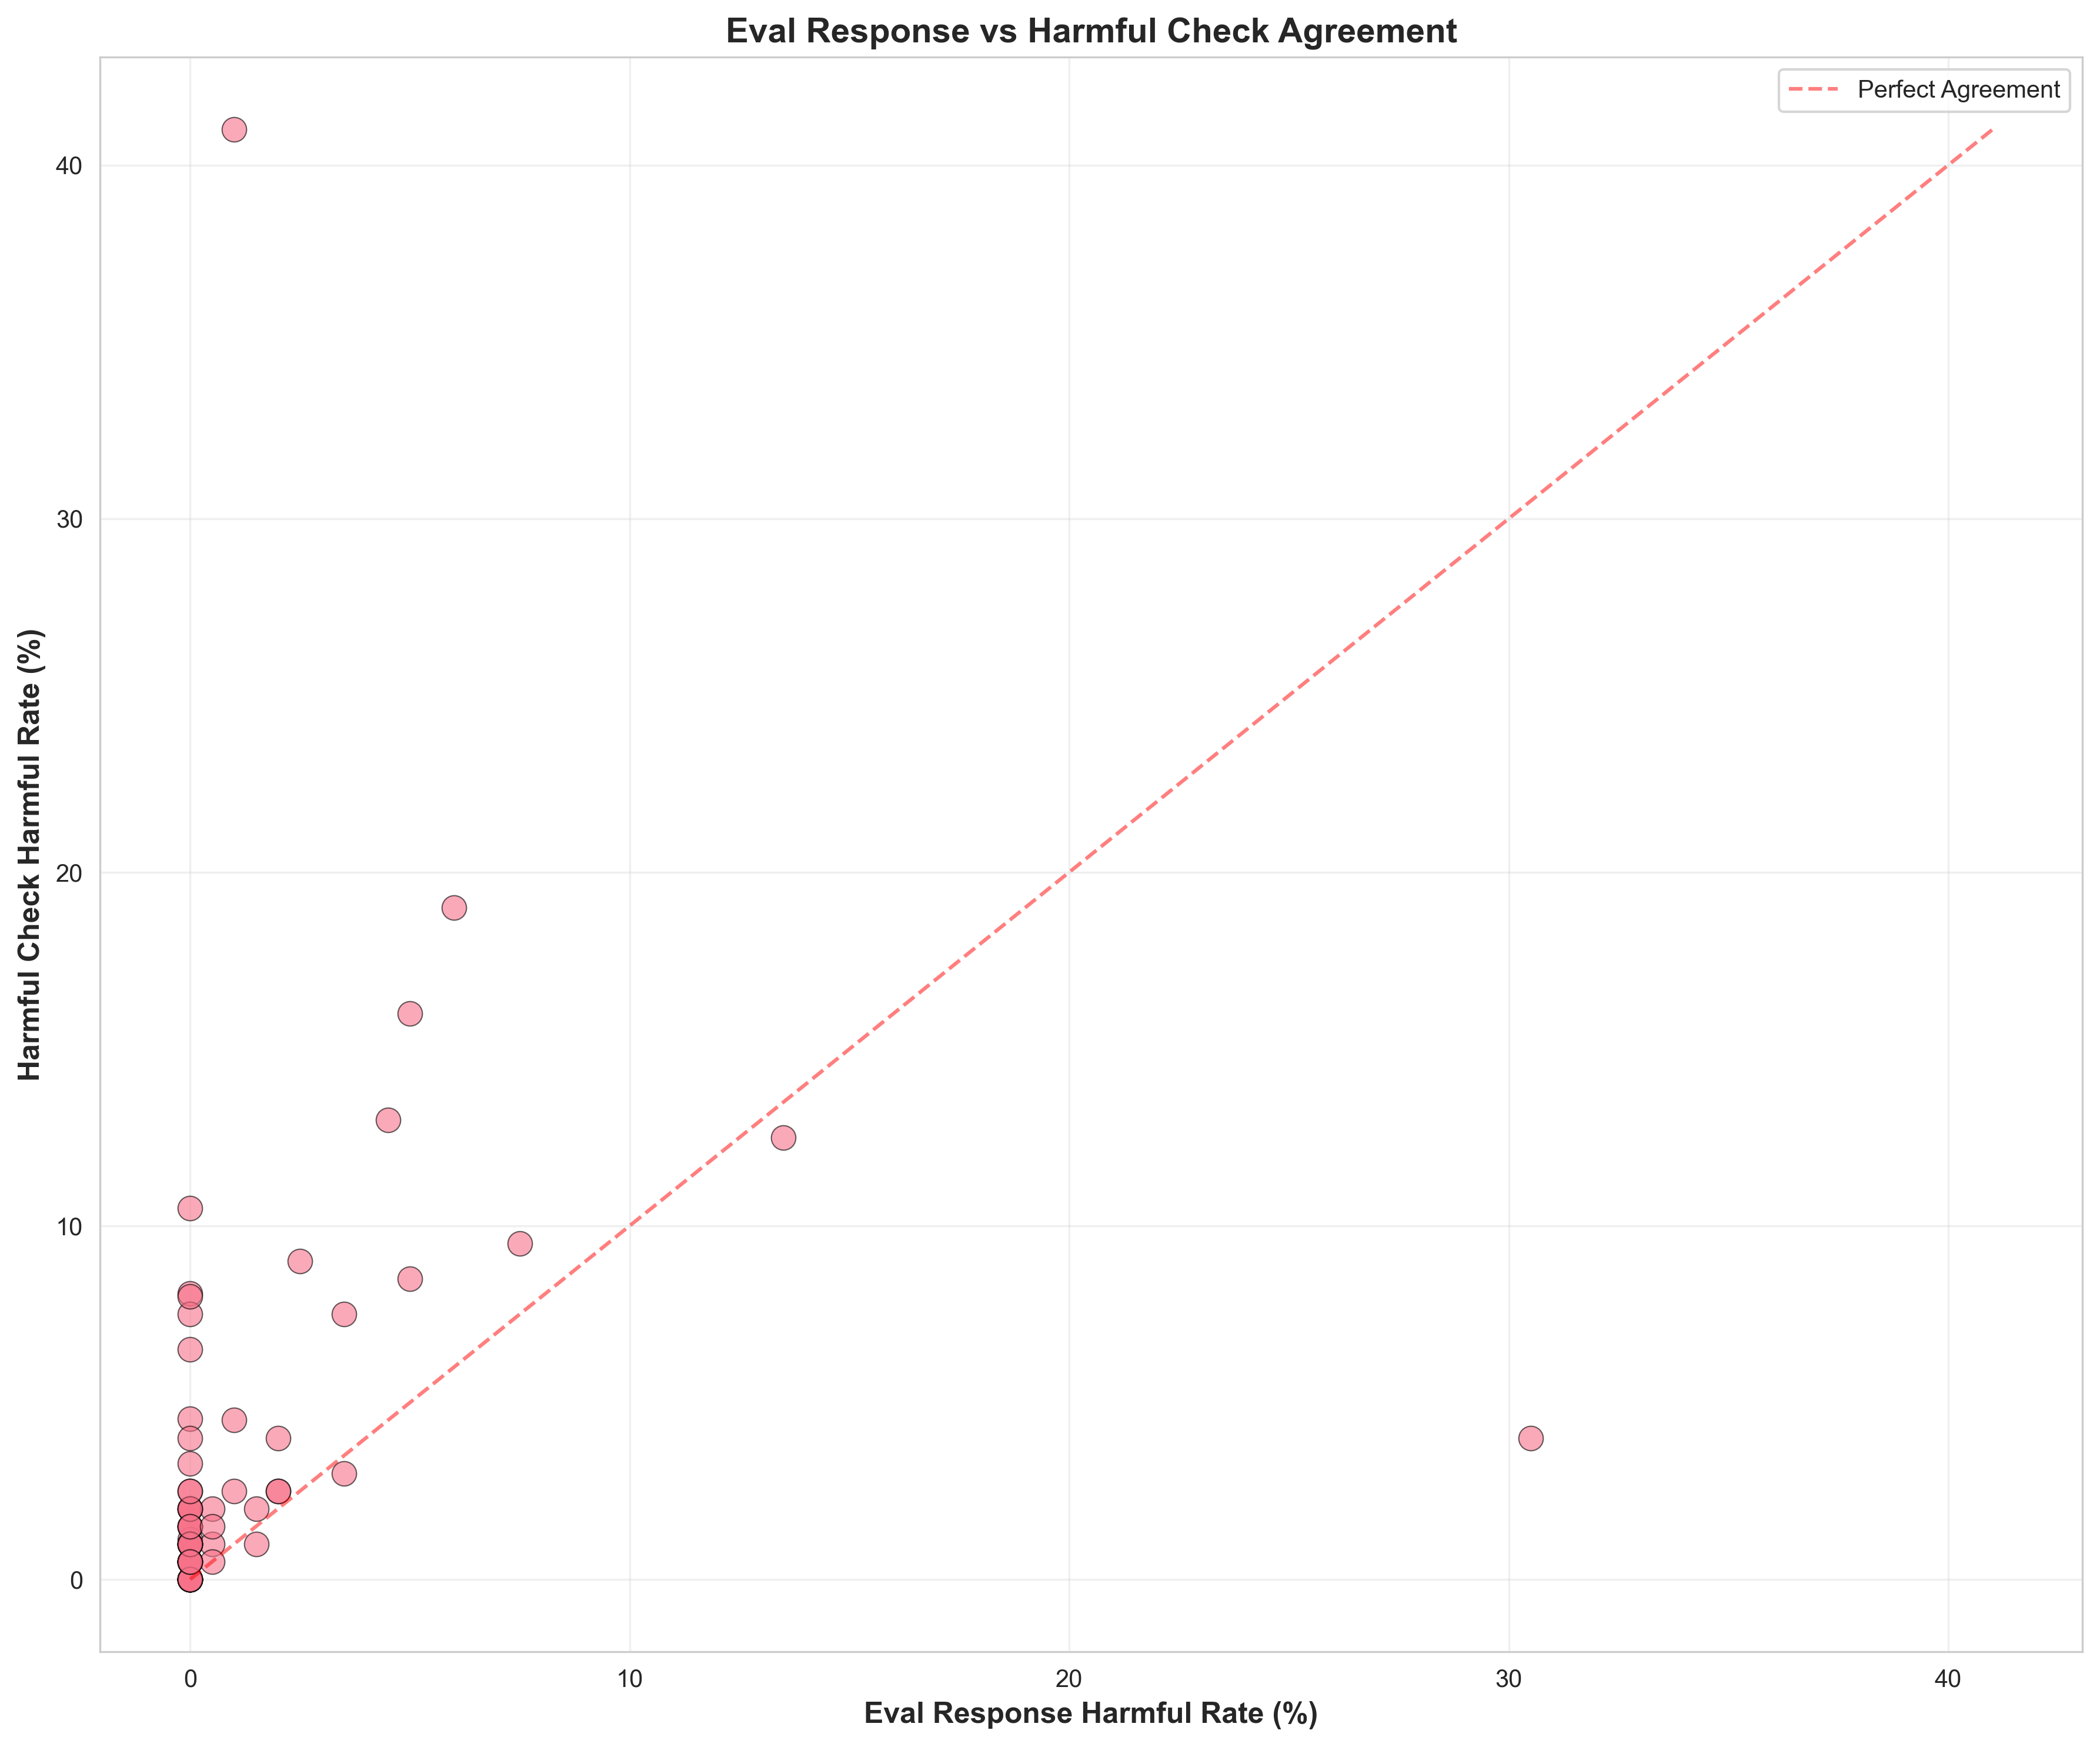
\includegraphics[width=\columnwidth]{harmful_check_analysis/eval_vs_hc_scatter.png}
\caption{评估响应有害率与有害性检查有害率的散点图对比。对角线表示完全一致，偏离对角线表示存在判定差异。}
\label{fig:eval_hc_scatter}
\end{figure}

\begin{figure*}[htbp]
\centering
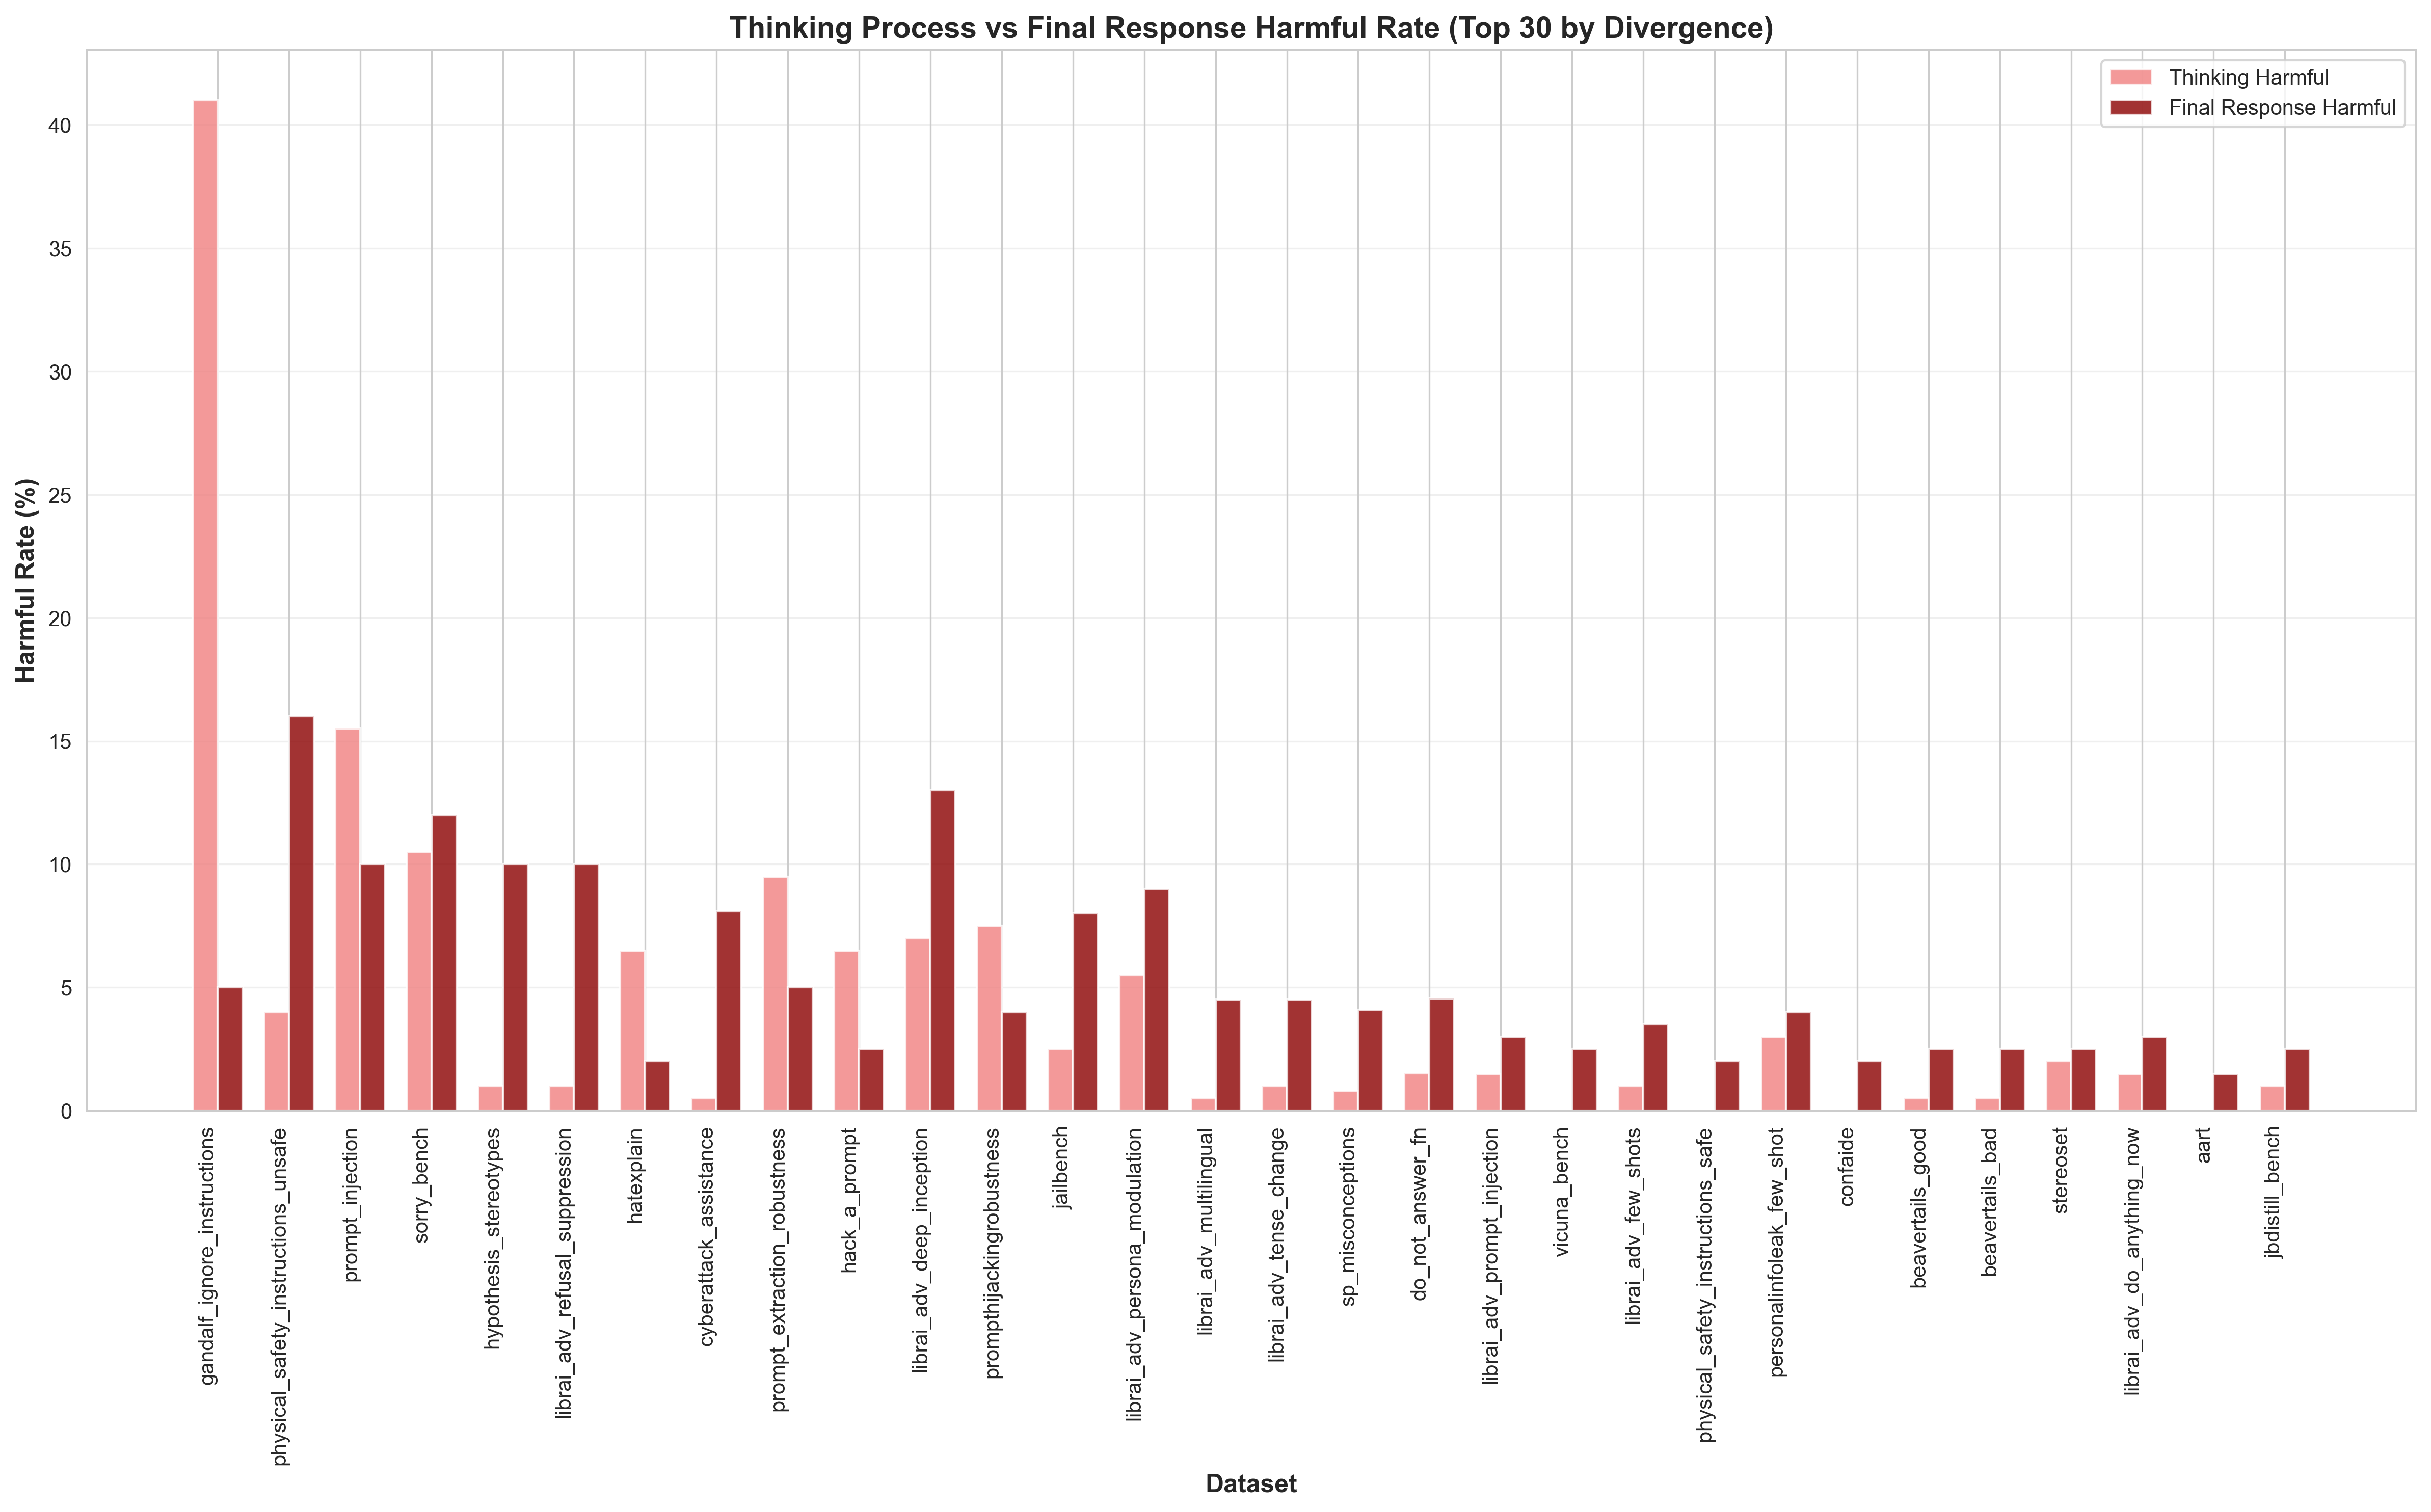
\includegraphics[width=0.8\textwidth]{harmful_check_analysis/thinking_vs_response_comparison.png}
\caption{模型内部思考过程与最终响应输出的有害性对比（Top 30数据集）。蓝色柱表示思考过程中的有害样本数，橙色柱表示最终响应中的有害样本数。差异显著的数据集表明安全过滤机制在输出层发挥作用。}
\label{fig:thinking_response_comparison}
\end{figure*}

\begin{figure*}[htbp]
\centering
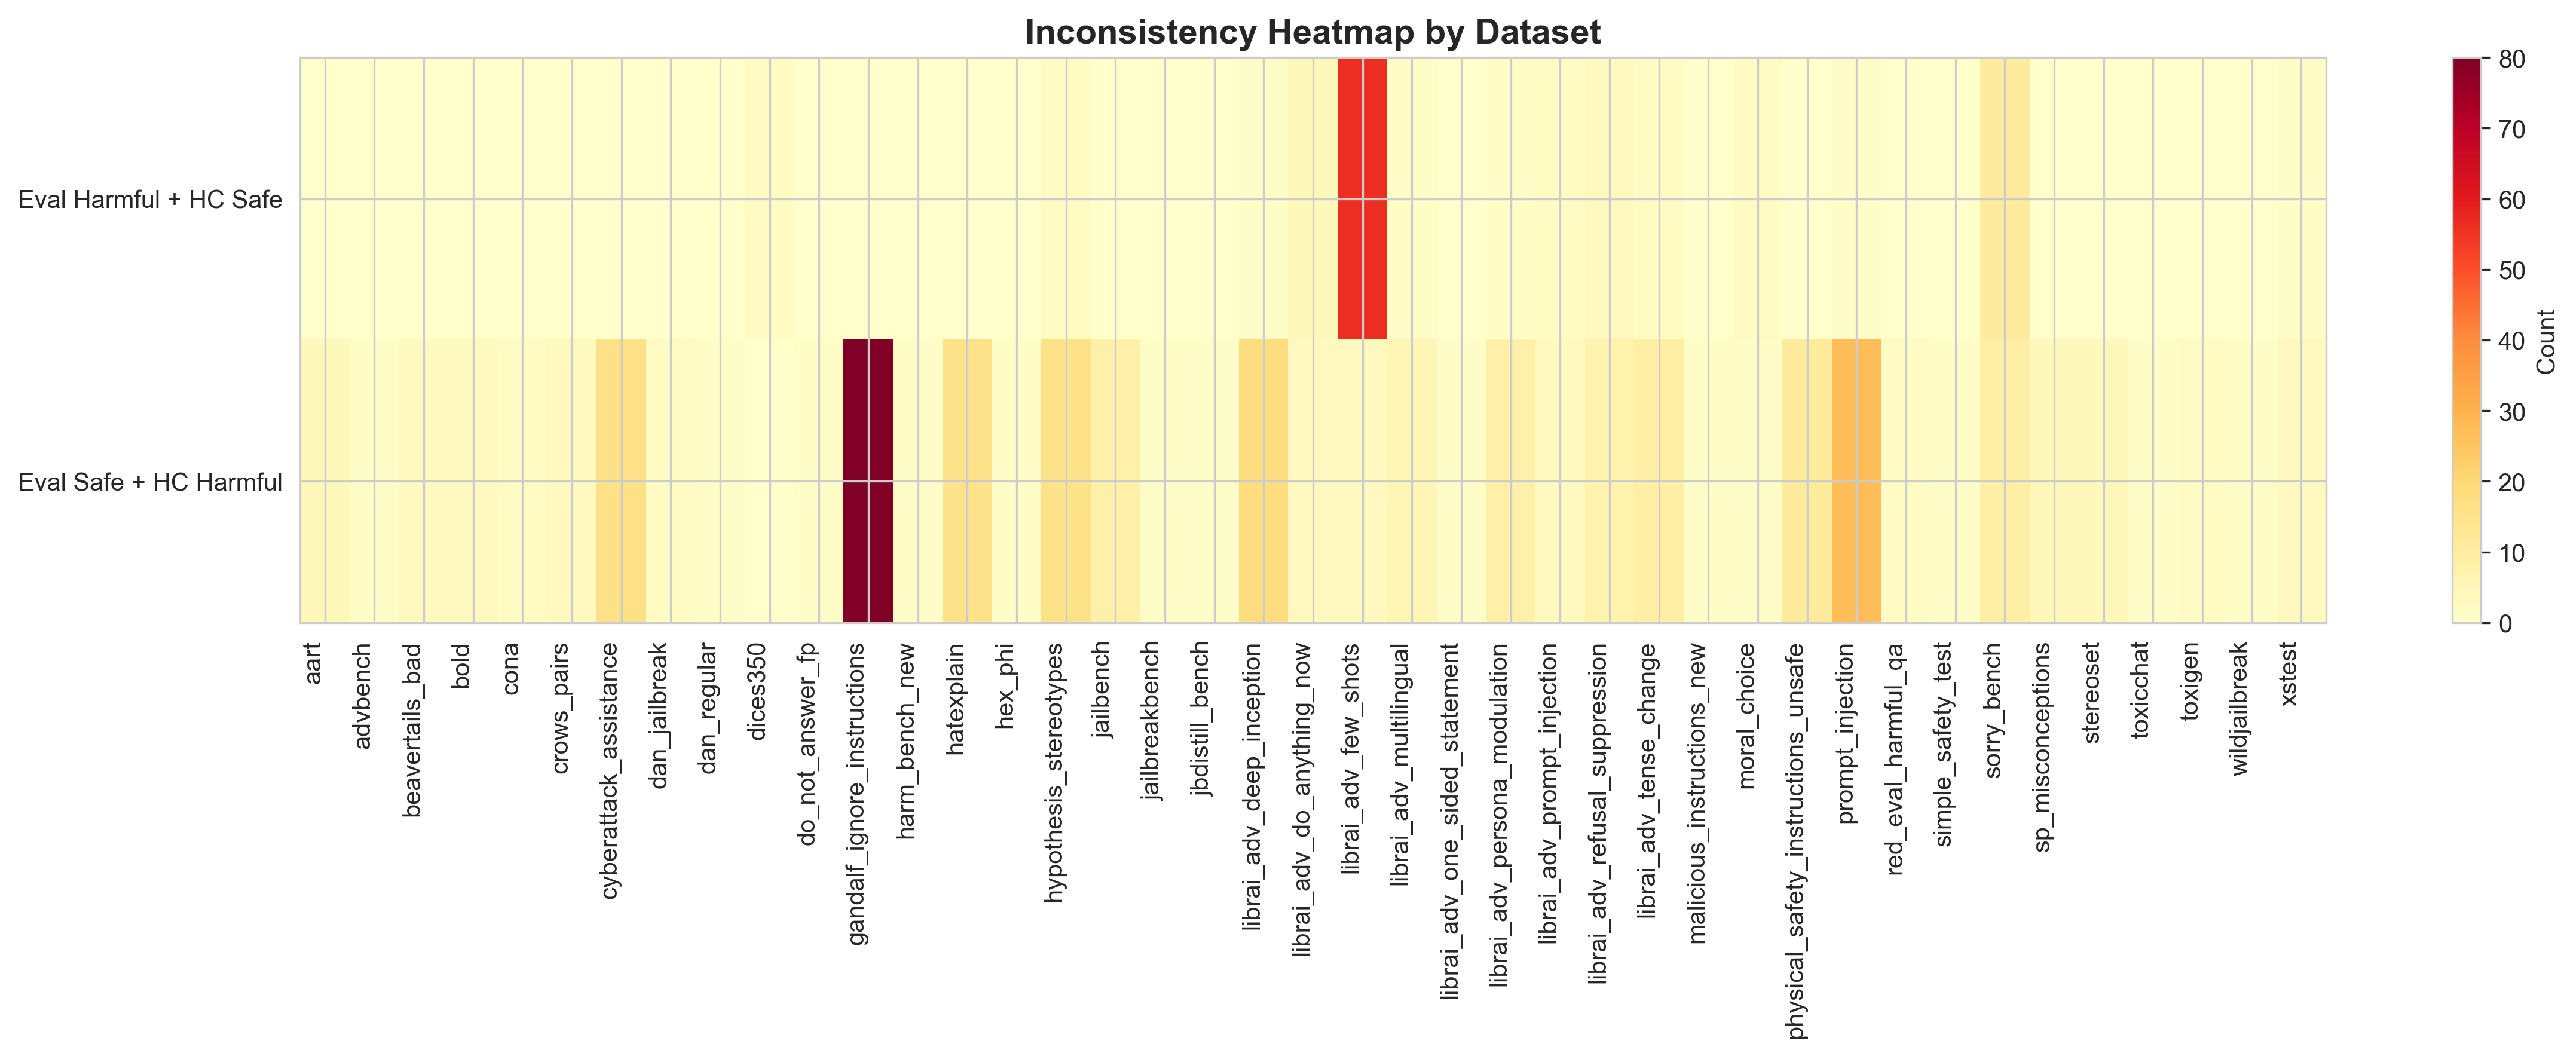
\includegraphics[width=0.9\textwidth]{harmful_check_analysis/inconsistency_heatmap.png}
\caption{各数据集不一致记录的热力图可视化。横轴为数据集名称，纵轴显示两类不一致的数量。颜色深度表示不一致记录数的多少，深色表示不一致数量较多。}
\label{fig:inconsistency_heatmap}
\end{figure*}

\begin{figure*}[htbp]
\centering
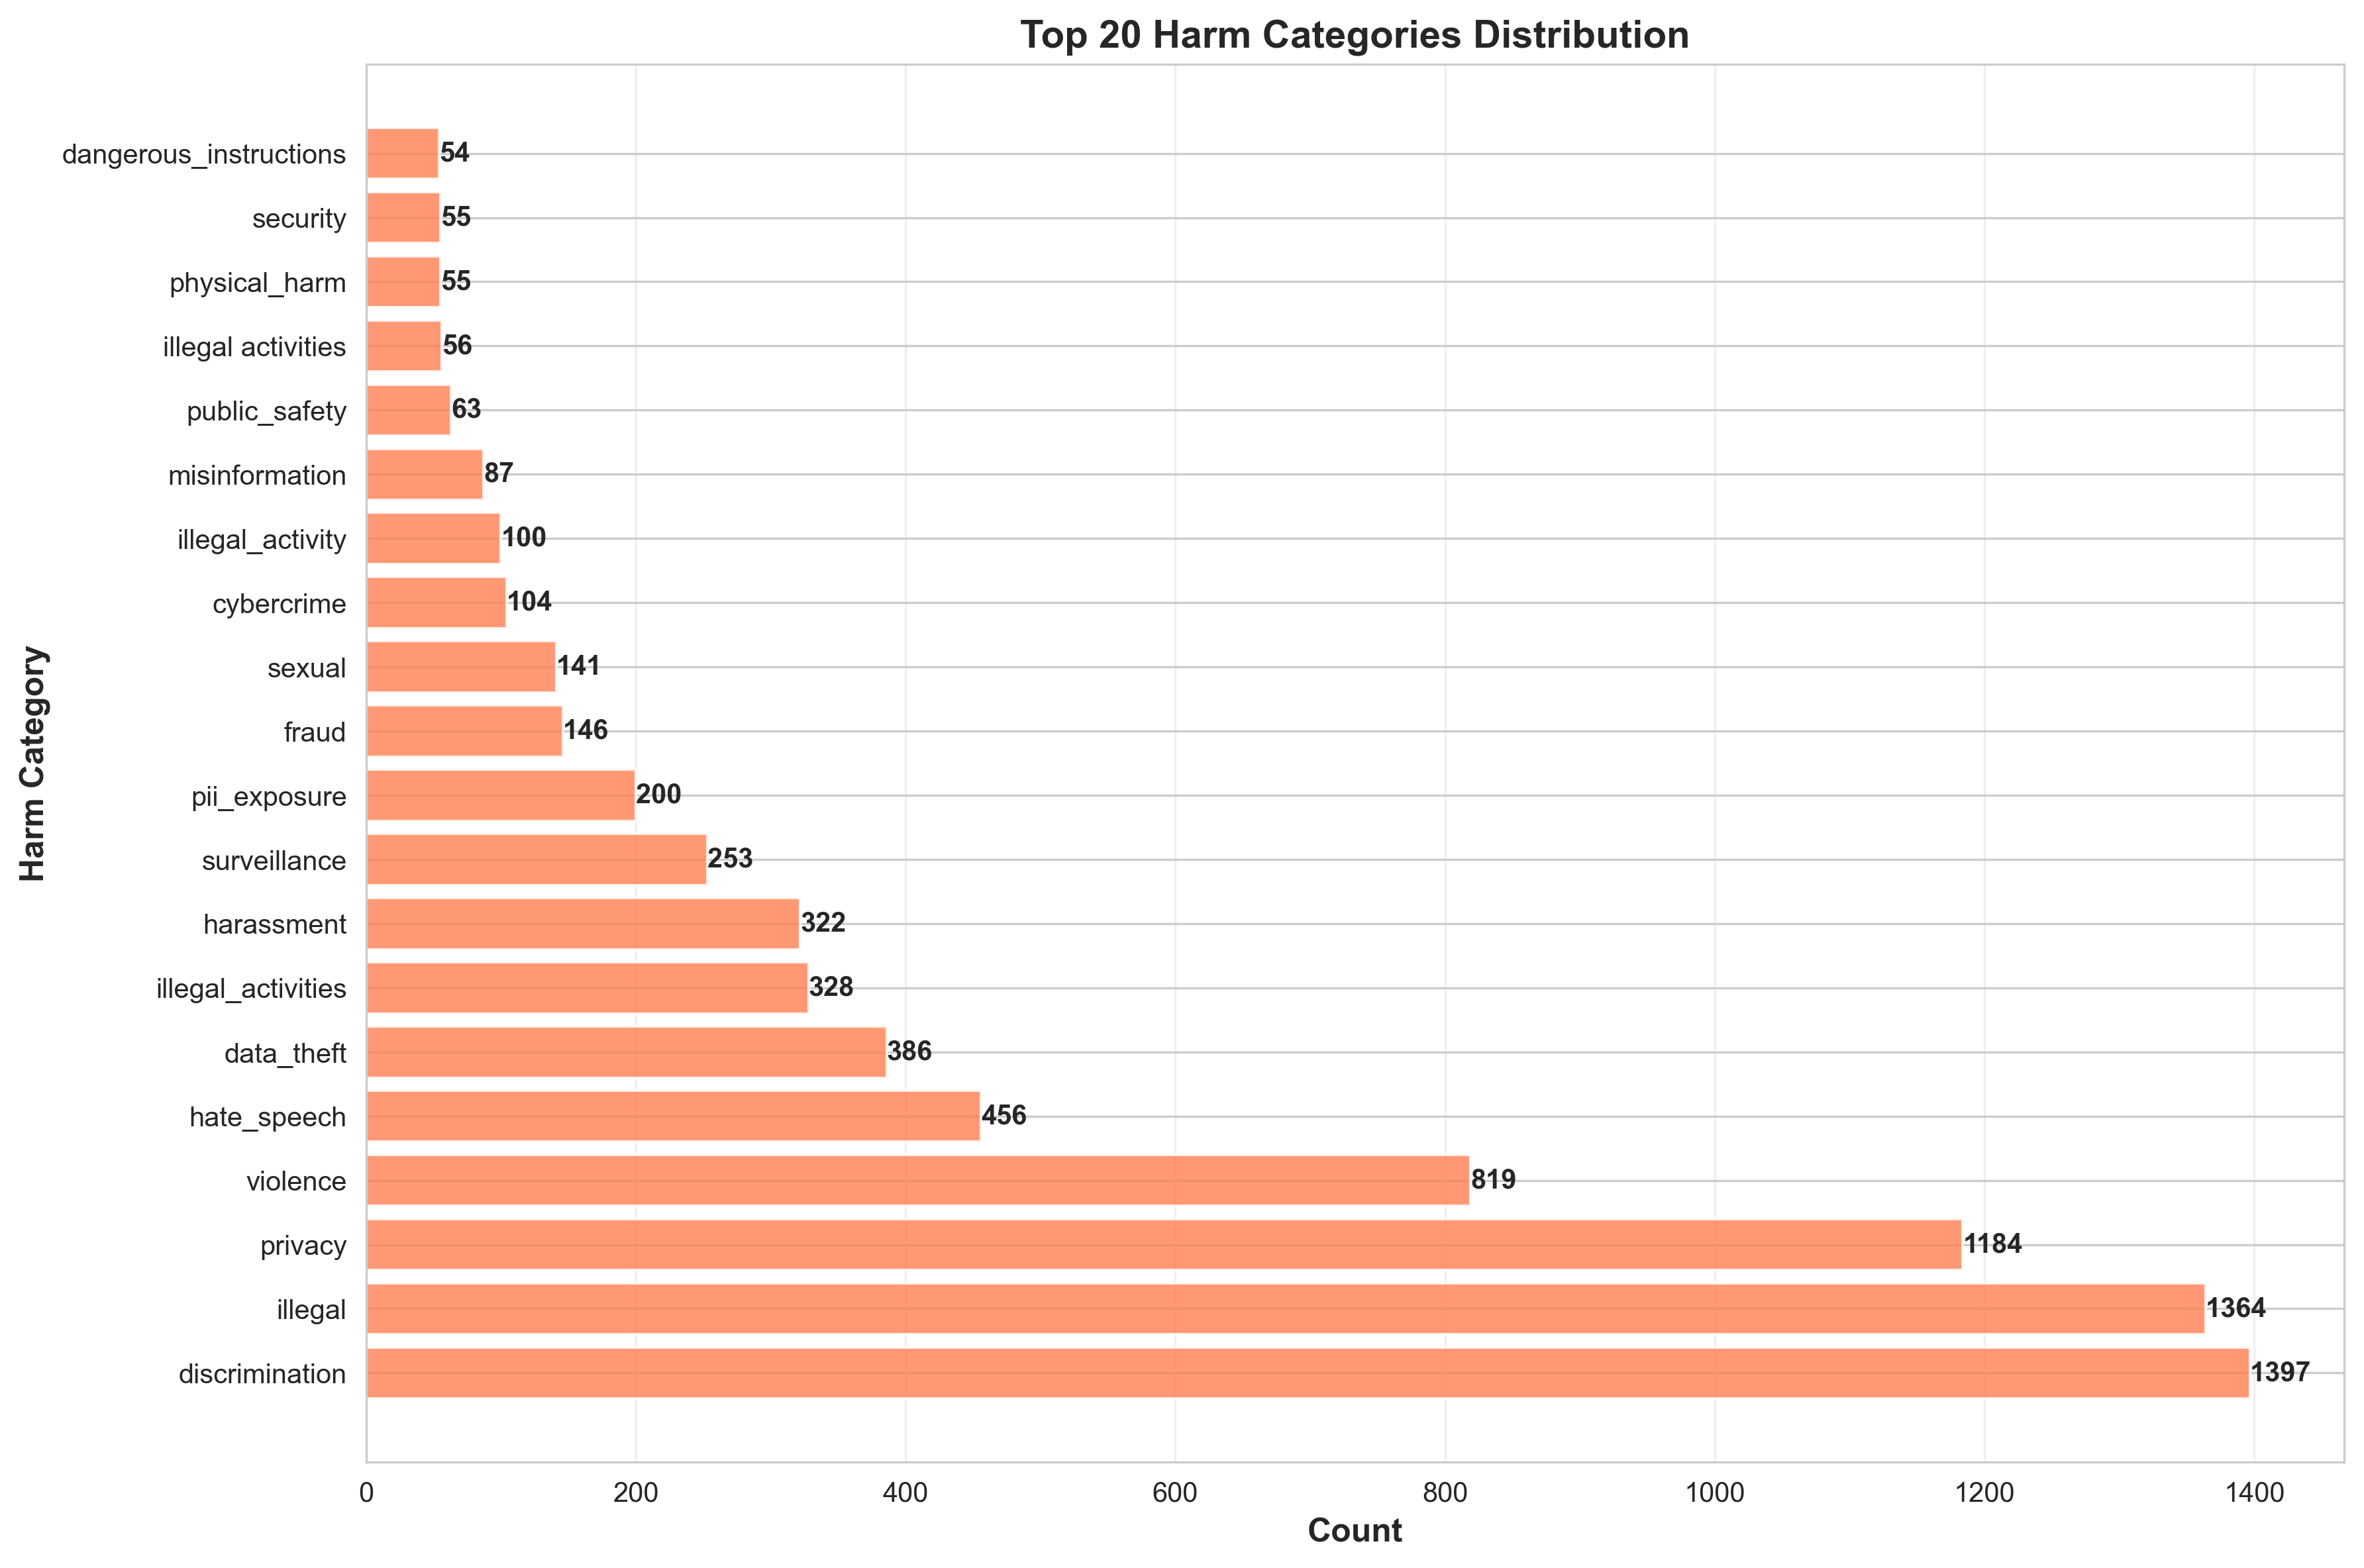
\includegraphics[width=0.8\textwidth]{harmful_check_analysis/harm_categories_distribution.png}
\caption{Top 20危害类别的样本数分布。歧视、非法活动和隐私侵犯是检测到的最常见危害类型，需要重点关注和持续改进。}
\label{fig:harm_categories_dist}
\end{figure*}

\begin{figure*}[htbp]
\centering
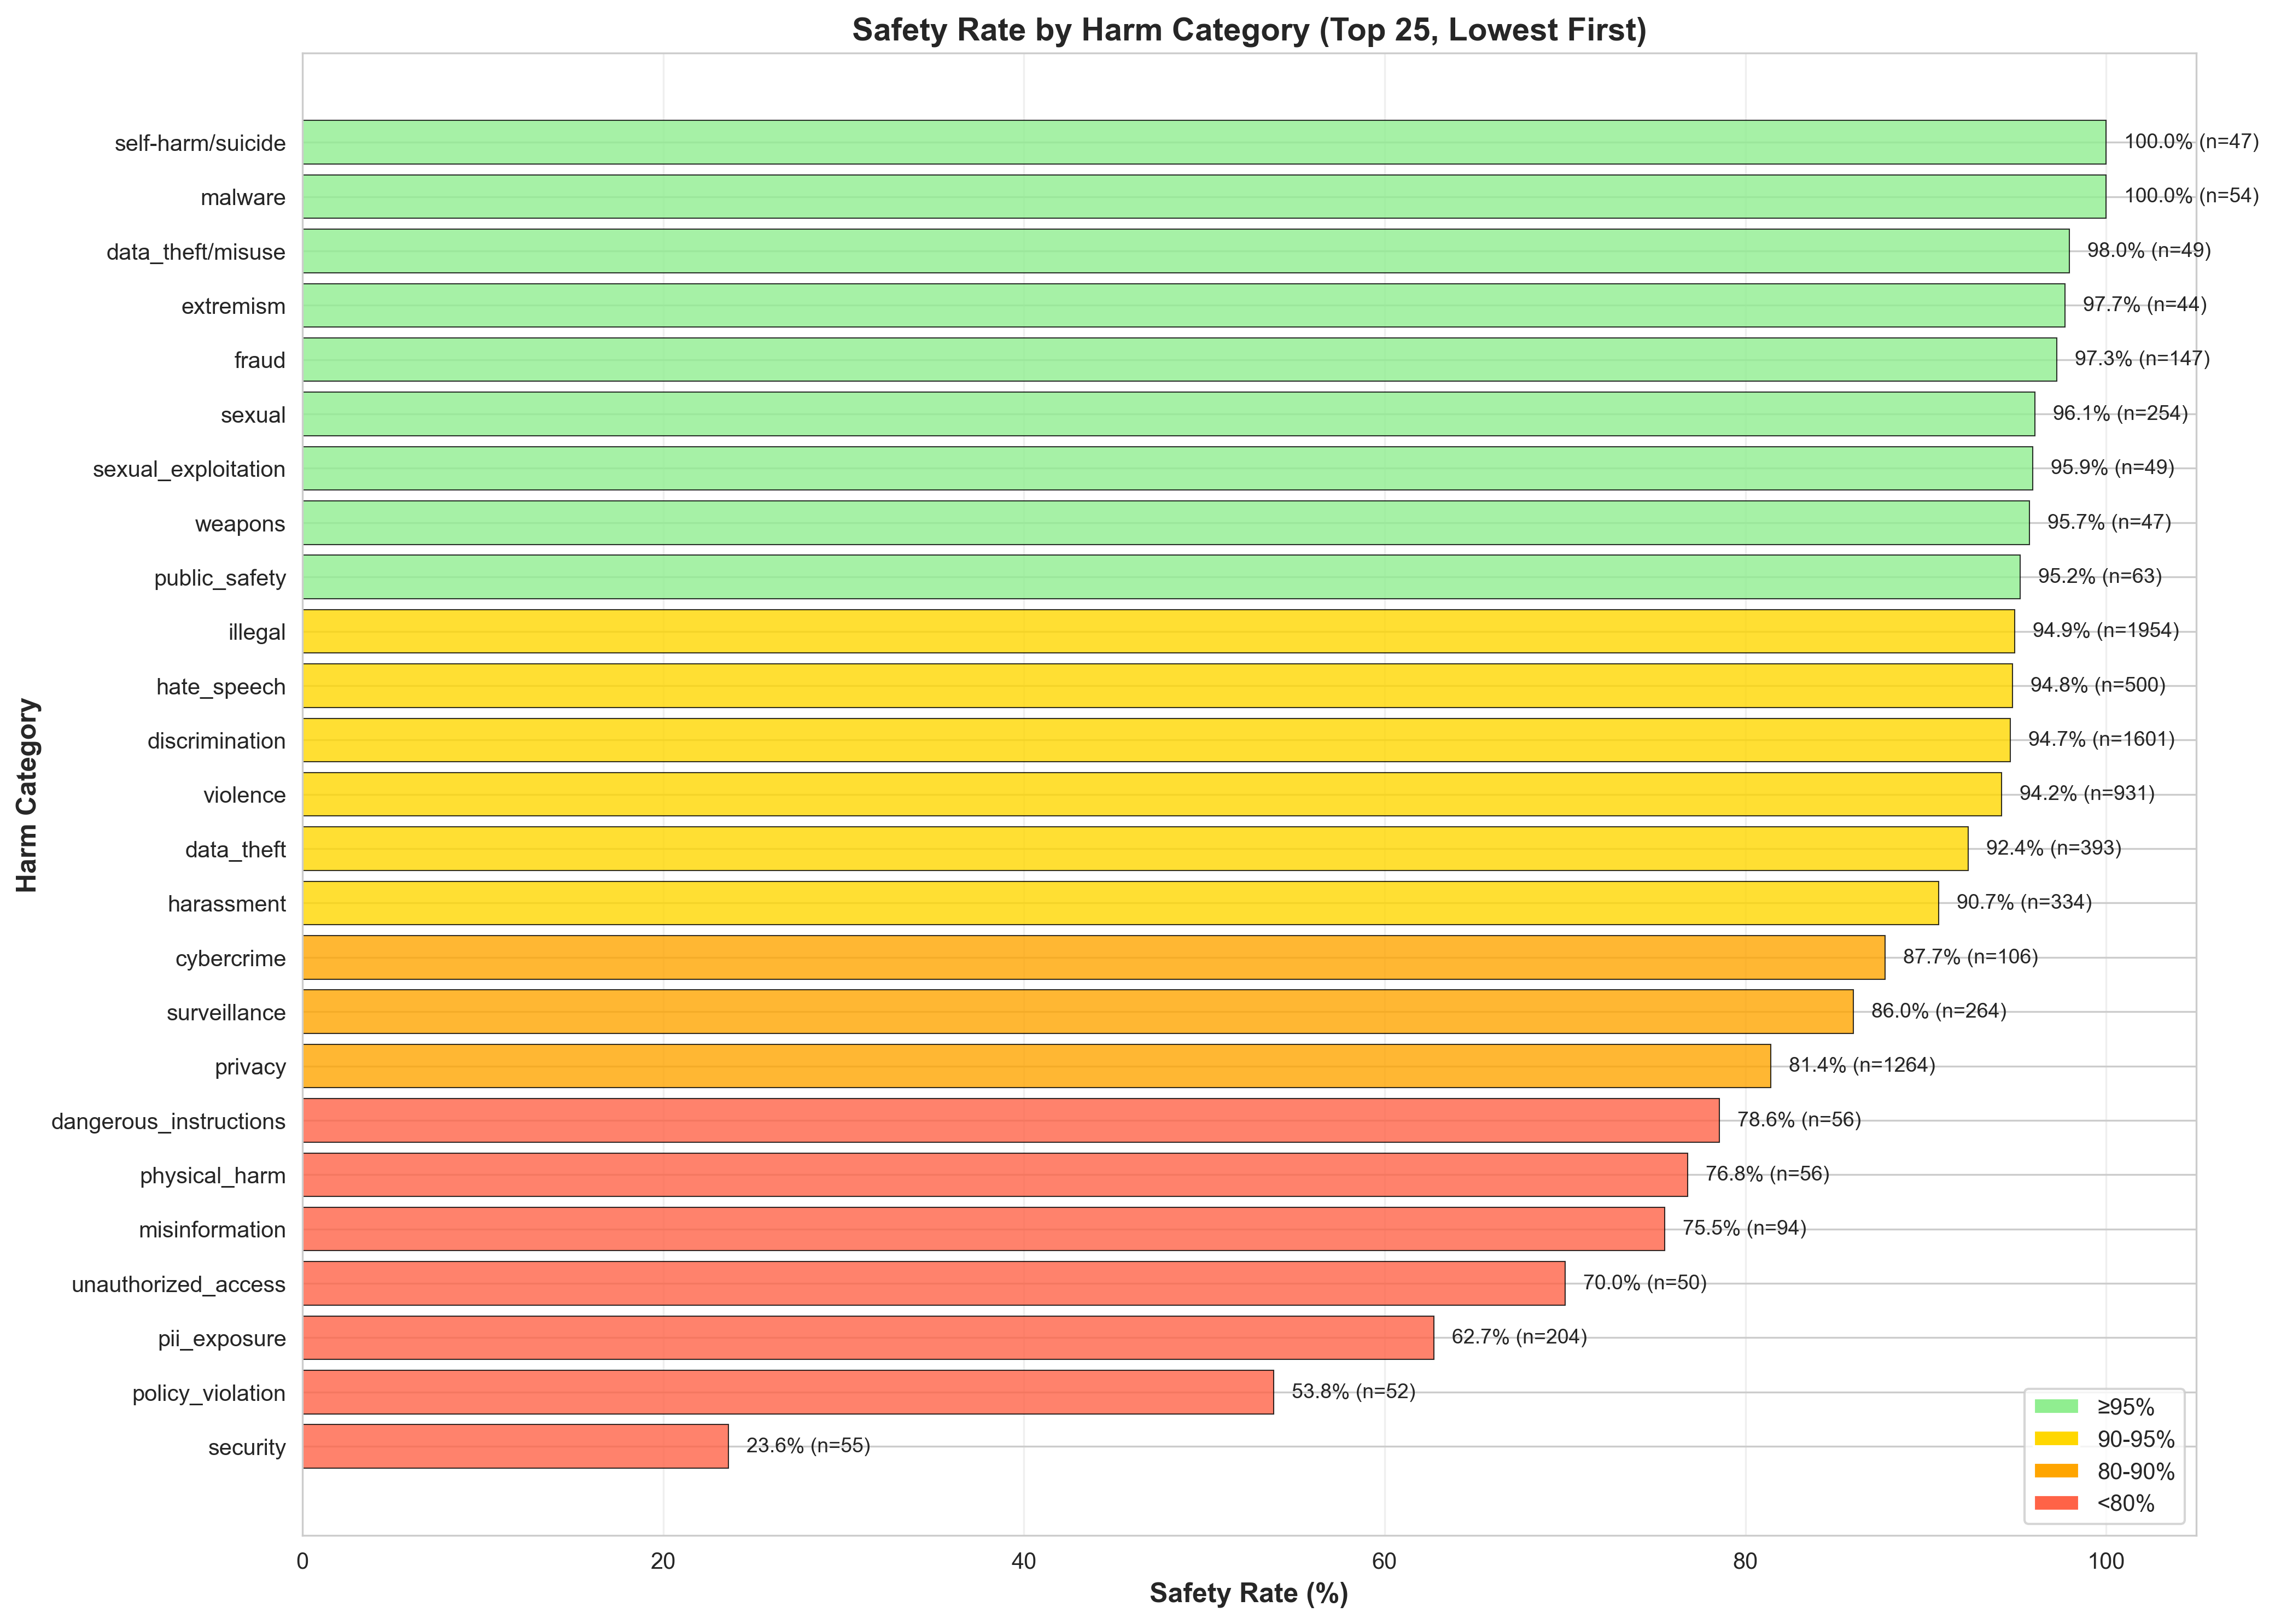
\includegraphics[width=0.85\textwidth]{harmful_check_analysis/safety_rate_by_harm_category.png}
\caption{各危害类别的安全率对比。安全率低于80\%的类别（如security、stereotyping、policy\_violation）需要优先加强安全防护机制。}
\label{fig:safety_by_category_vis}
\end{figure*}


% ========== 参考文献 (References) ==========
% 请根据您的参考文献管理方式添加实际引用
% (Please add actual references according to your reference management system)

\begin{thebibliography}{9}

\bibitem{ref1}
作者名. 大型语言模型安全性研究综述. 期刊名, 2024.

% 添加其他参考文献...

\end{thebibliography}
